\documentclass[12pt,a4paper]{article}

% ─── Page Layout ───────────────────────────────────────────────────────────────
\usepackage[a4paper, margin=0.8in, headheight=14pt]{geometry}

% ─── Fonts (XeLaTeX) ───────────────────────────────────────────────────────────
\usepackage{fontspec}
\usepackage{unicode-math}
\setmainfont{TeX Gyre Pagella}
\setmonofont[Scale=0.88]{TeX Gyre Cursor}
\setmathfont{Latin Modern Math}

% ─── Packages ──────────────────────────────────────────────────────────────────
\usepackage{xcolor}
\usepackage{colortbl}
\usepackage{titlesec}
\usepackage{enumitem}
\usepackage{tabularx}
\usepackage{longtable}
\usepackage{booktabs}
\usepackage{array}
\usepackage{amsmath}
\usepackage{tikz}
\usetikzlibrary{shapes.geometric, arrows.meta, positioning, calc, fit, decorations.pathreplacing, patterns}
\usepackage{tcolorbox}
\tcbuselibrary{skins, breakable}
\usepackage{hyperref}
\usepackage{fancyhdr}
\usepackage{graphicx}
\usepackage{microtype}
\hyphenpenalty=10000
\exhyphenpenalty=10000
\sloppy
\usepackage{caption}
\usepackage{setspace}
\usepackage{multirow}
\usepackage{tocloft}

% ─── Q&A helper ────────────────────────────────────────────────────────────────
\newcommand{\Q}[1]{\textbf{#1}\par\noindent\ignorespaces}

% ─── Colour Palette ────────────────────────────────────────────────────────────
\definecolor{myred}{RGB}{196,30,58}
\definecolor{mydark}{RGB}{30,30,50}
\definecolor{mygreen}{RGB}{14,120,80}
\definecolor{myteal}{RGB}{0,130,140}
\definecolor{myamber}{RGB}{180,100,0}
\definecolor{mypurple}{RGB}{100,30,160}
\definecolor{mygray}{RGB}{246,247,249}
\definecolor{mgframe}{RGB}{180,185,200}
\definecolor{watermark}{RGB}{145,150,170}
\definecolor{hdrred}{RGB}{250,232,235}
\definecolor{hdrgreen}{RGB}{220,244,233}
\definecolor{hdrteal}{RGB}{220,242,244}
\definecolor{hdramber}{RGB}{253,242,215}
\definecolor{hdrpurple}{RGB}{238,228,255}
\definecolor{hdrgray}{RGB}{238,240,245}

% ─── Section Formatting ────────────────────────────────────────────────────────
\titleformat{\section}
  {\large\bfseries\color{myred}}{\thesection.}{0.5em}{}
  [\vspace{1pt}{\color{myred}\rule{\linewidth}{0.8pt}}]
\titleformat{\subsection}
  {\normalsize\bfseries\color{myteal}}{\thesubsection}{0.5em}{}
\titlespacing*{\section}{0pt}{18pt}{7pt}
\titlespacing*{\subsection}{0pt}{11pt}{4pt}

% ─── Paragraph ─────────────────────────────────────────────────────────────────
\setlength{\parindent}{0pt}
\setlength{\parskip}{4pt}

% ─── TOC Styling ───────────────────────────────────────────────────────────────
\renewcommand{\cfttoctitlefont}{\large\bfseries\color{myred}}
\renewcommand{\cftaftertoctitle}{\par\noindent{\color{myred}\rule{\linewidth}{0.8pt}}}
\setlength{\cftbeforetoctitleskip}{0pt}
\setlength{\cftaftertoctitleskip}{6pt}
\renewcommand{\cftsecfont}{\normalsize\bfseries\color{mydark}}
\renewcommand{\cftsecpagefont}{\normalsize\bfseries\color{mydark}}
\renewcommand{\cftsecleader}{\cftdotfill{\cftdotsep}}
\setlength{\cftbeforesecskip}{7pt}
\renewcommand{\cftsubsecfont}{\small\color{mydark}}
\renewcommand{\cftsubsecpagefont}{\small\color{mydark}}
\setlength{\cftbeforesubsecskip}{3pt}
\setlength{\cftsubsecindent}{1.4em}

% ─── Table helpers ─────────────────────────────────────────────────────────────
\renewcommand{\arraystretch}{1.45}
\setlength{\tabcolsep}{6pt}
\arrayrulecolor{mydark}
\newcolumntype{B}[1]{>{\small\bfseries\raggedright\arraybackslash}m{#1}}
\newcolumntype{Y}{>{\small\raggedright\arraybackslash}X}
\renewcommand{\tabularxcolumn}[1]{m{#1}}

% ─── Header / Footer ───────────────────────────────────────────────────────────
\pagestyle{fancy}
\fancyhf{}
\fancyhead[L]{\small\color{myred}\textbf{ES-CS401}\;\color{mydark}--- Design and Analysis of Algorithms}
\fancyhead[R]{\small\color{myteal}\textbf{Module 5 Notes}}
\fancyfoot[C]{\small\color{mydark}\thepage}
\fancyfoot[R]{\small\color{watermark}\textit{\copyright\ Biraj Sarkar (CGEC)}}
\renewcommand{\headrulewidth}{0.5pt}
\renewcommand{\footrulewidth}{0.3pt}

% ─── Hyperref ──────────────────────────────────────────────────────────────────
\hypersetup{
  colorlinks=true, linkcolor=myteal, urlcolor=myteal,
  pdfauthor={Biraj Sarkar (CGEC)},
  pdftitle={ES-CS401 --- Module 5 Notes: Approximation, Randomization and PSPACE}
}

% ─── tcolorbox styles ──────────────────────────────────────────────────────────
\tcbset{
  tikzbox/.style={
    colback=mygray, colframe=mgframe, boxrule=0.6pt, arc=4pt,
    left=8pt, right=8pt, top=6pt, bottom=6pt,
    colbacktitle=mgframe, coltitle=mydark, fonttitle=\small\bfseries
  },
  defbox/.style={
    colback=hdrgreen, colframe=mygreen, boxrule=0.8pt, arc=4pt,
    left=9pt, right=9pt, top=6pt, bottom=6pt,
    colbacktitle=mygreen, coltitle=white, fonttitle=\small\bfseries
  },
  formulabox/.style={
    colback=hdrteal, colframe=myteal, boxrule=0.8pt, arc=4pt,
    left=9pt, right=9pt, top=7pt, bottom=7pt,
    colbacktitle=myteal, coltitle=white, fonttitle=\small\bfseries
  },
  examplebox/.style={
    colback=hdramber, colframe=myamber, boxrule=0.8pt, arc=4pt,
    left=9pt, right=9pt, top=6pt, bottom=6pt,
    colbacktitle=myamber, coltitle=white, fonttitle=\small\bfseries
  },
  masonbox/.style={
    colback=hdrpurple, colframe=mypurple, boxrule=0.8pt, arc=4pt,
    left=9pt, right=9pt, top=6pt, bottom=6pt,
    colbacktitle=mypurple, coltitle=white, fonttitle=\small\bfseries
  },
  exambox/.style={
    colback=hdrpurple, colframe=mypurple, boxrule=1pt, arc=5pt,
    left=10pt, right=10pt, top=8pt, bottom=8pt,
    colbacktitle=mypurple, coltitle=white, fonttitle=\bfseries,
    breakable, title after break={\textbf{Frequently Asked / Viva Questions (contd.)}}
  }
}
\tcbset{breakable}
\tcbset{after={\par\color{black}}}

% ─── TikZ styles ───────────────────────────────────────────────────────────────
\tikzset{
  block/.style={rectangle, draw=myteal, fill=hdrteal,
    text width=2.4cm, align=center, minimum height=0.95cm,
    font=\small, rounded corners=3pt, line width=0.7pt},
  redblock/.style={rectangle, draw=myred, fill=hdrred,
    text width=2.4cm, align=center, minimum height=0.95cm,
    font=\small, rounded corners=3pt, line width=0.7pt},
  amberblock/.style={rectangle, draw=myamber, fill=hdramber,
    text width=2.4cm, align=center, minimum height=0.95cm,
    font=\small, rounded corners=3pt, line width=0.7pt},
  sumjunc/.style={circle, draw=myamber, fill=hdramber,
    minimum size=0.62cm, font=\small, line width=0.8pt},
  arrow/.style={-Stealth, thick, color=mydark},
  redarrow/.style={-Stealth, thick, color=myred},
  line/.style={thick, color=mydark}
}

\begin{document}

% ─── Title Page ───────────────────────────────────────────────────────────────
\begin{center}
  {\LARGE\bfseries\color{myred} ES-CS401 --- Design and Analysis of Algorithms}\\[5pt]
  {\normalsize\color{mydark} Semester IV \quad$\bullet$\quad 3L:0T:0P \quad$\bullet$\quad 3 Credits}\\[3pt]
  {\normalsize\color{myteal}\textbf{Module 5 Exam Notes: Approximation, Randomization and PSPACE}}\\[3pt]
  {\small\color{mydark} CGEC \;$|$\; B.Tech ECE (2023--27) \;$|$\; \textit{Biraj Sarkar}}
\end{center}
\vspace{2pt}
\noindent{\color{myred}\rule{\linewidth}{1.5pt}}
\vspace{2pt}

\hypersetup{linkcolor=mydark}
\tableofcontents
\hypersetup{linkcolor=myteal}
\newpage

\section{Approximation, Randomization and PSPACE}
\subsection{Approximation ratios and algorithm families}
\begin{tcolorbox}[defbox, title={Approximation algorithm}]
An \textbf{approximation algorithm} constructs a feasible solution in polynomial time and has a proved bound on how far its value can be from the optimum. The ratio is meaningful under the specified input and objective assumptions. A heuristic may be effective in practice without a proved ratio.
\end{tcolorbox}

\begin{tcolorbox}[formulabox, title={Ratio convention for nonnegative objectives}]
Write $A(I)$ for the algorithm's objective value and $\mathrm{OPT}(I)$ for the optimal value. For $\rho\ge1$, guarantee
\[
\begin{array}{ll}
A(I)\le\rho\,\mathrm{OPT}(I), & \text{minimisation},\\
A(I)\ge\mathrm{OPT}(I)/\rho, & \text{maximisation}.
\end{array}
\]
These inequalities also state what must happen when either value is zero. Some texts report the reciprocal ratio for maximisation.
\end{tcolorbox}

\par\vspace{5pt}
\begingroup
\setlength{\extrarowheight}{1pt}
\noindent\begin{tabularx}{\linewidth}{|B{3.5cm}|Y|Y|}
\hline
\textbf{Guarantee} & \textbf{What is promised} & \textbf{Runtime qualification} \\ \hline
Constant factor & A fixed $\rho$, for example $2$. & Polynomial in the input length. \\ \hline
PTAS & A family with ratio $1+\varepsilon$ for any fixed $\varepsilon>0$. & Polynomial in input length for each fixed accuracy. The exponent may depend on accuracy. \\ \hline
FPTAS & A family with the same adjustable ratio. & Polynomial in both input length and $1/\varepsilon$. \\ \hline
\end{tabularx}\par
\endgroup
\textbf{Design pattern.} Find an efficiently computable lower bound for minimisation, or an upper bound for maximisation. Compare the output against it. Be explicit about feasibility and all assumptions used in the proof.

\subsection{Worked scheme: value scaling for zero-one knapsack}
\begin{tcolorbox}[examplebox, title={Why value scaling gives an FPTAS}]
Discard items that individually exceed the capacity. Let $n$ be the remaining item count and $V_{\max}$ the largest remaining value. If every feasible value is zero or no item remains, return the empty set. Otherwise, choose a loss tolerance $0<\delta<1$. Set $K=\delta V_{\max}/n$ and replace item value $v_i$ by $q_i=\lfloor v_i/K\rfloor$. Keep the original weights.

\textbf{Solve the scaled problem.} For each total scaled value, store the minimum weight that attains it. Initially only value $0$ has finite weight. For each item compare skipping it with adding its weight to the previous state at scaled value $q-q_i$. Keep the largest scaled total whose weight stays within capacity and recover its chosen items.

\textbf{Bound the loss.} Let $S^*$ be an optimal original selection and $S$ the selection found by the scaled DP. Because $S$ maximises the scaled objective,
\begin{align*}
v(S)&\ge K\sum_{i\in S}q_i\\
    &\ge K\sum_{i\in S^*}q_i\\
    &\ge \mathrm{OPT}-nK\\
    &\ge (1-\delta)\,\mathrm{OPT}.
\end{align*}
The last line uses $V_{\max}\le\mathrm{OPT}$, since the most valuable remaining item fits by itself. For the reciprocal convention, choose $\delta=\varepsilon/(1+\varepsilon)$ to get $v(S)\ge\mathrm{OPT}/(1+\varepsilon)$.

Each $q_i\le n/\delta$, so there are $O(n^2/\delta)$ scaled totals. The DP uses $O(n^3/\delta)$ transitions, polynomial in both the input length and $1/\delta$.
\end{tcolorbox}

\subsection{Two-approximation for minimum vertex cover}
\begin{tcolorbox}[formulabox, title={Maximal-matching algorithm for vertex cover}]
\begin{verbatim}
Set cover = empty.
While an uncovered edge (u, v) remains:
    add u and v to cover
    delete all edges incident to u or v
Return cover.
\end{verbatim}
\end{tcolorbox}

The selected edges form a \emph{maximal} matching $M$. No two selected edges share an endpoint, and an additional disjoint edge would have survived the deletions. Every edge is covered when none remains. Every vertex cover uses at least one endpoint per edge of $M$, so
\[
|C|=2|M|\le 2\,\mathrm{OPT}.
\]
The implementation can scan the edges once and select both endpoints just when neither has been selected. It uses $O(V+E)$ time with vertex marks.
\begin{tcolorbox}[examplebox, title={A cover can attain exactly twice the optimum}]
In a star with centre $a$ and leaves $b,c,d$, selecting edge $ab$ includes both $a$ and $b$ and finishes. The optimum is $\{a\}$. Thus this instance makes the guarantee tight.
\end{tcolorbox}

\subsection{Metric TSP and bin packing guarantees}
\begin{enumerate}[leftmargin=*, itemsep=3pt, topsep=4pt]
  \item \textbf{Find an MST.} Removing one edge from an optimal tour leaves a spanning tree, so the MST cost is no more than the optimum.
  \item \textbf{Double each tree edge.} Every vertex then has even degree, producing a closed Euler tour of weight twice the MST.
  \item \textbf{Shortcut repeated vertices.} Retain each vertex on its first visit and return to the start. By the triangle inequality, every shortcut costs no more than the portion it replaces.
  \item \textbf{Combine the bounds.} The resulting Hamiltonian tour costs at most twice the MST weight and hence at most twice the optimal tour weight.
\end{enumerate}
This proof assumes a complete symmetric graph of nonnegative metric costs. For unrelated weights, a shortcut may be arbitrarily expensive.
\begin{tcolorbox}[examplebox, title={Double-tree tour on a unit square}]
Let $A,B,C,D$ be the vertices in clockwise order. The MST can be $AB,BC,CD$ of total cost $3$. The doubled traversal $A,B,C,D,C,B,A$ costs $6$. Shortcut the repeated visits to get $A,B,C,D,A$ of cost $4$. Every tour needs four edges of cost at least $1$, so this particular tour is optimal.
\end{tcolorbox}

\textbf{Next Fit for bin packing.} When an item opens a new bin, it did not fit in the previous bin. Any two consecutive bins therefore have total load exceeding one bin capacity. Pair bins $(1,2),(3,4),\dots$. If $k\ge2$ bins are opened at capacity $C$, the total volume exceeds $\lfloor k/2\rfloor C$. Thus $\mathrm{OPT}\ge\lfloor k/2\rfloor+1$ and $k\le2\,\mathrm{OPT}-1$. The result also holds for a single nonempty bin. Next Fit uses $O(n)$ time. Module 2 compares practical placement rules such as First Fit and First Fit Decreasing.

\section{Randomized Algorithms}
\subsection{Random choices, expectation and error}
\begin{tcolorbox}[defbox, title={Randomized algorithm}]
A randomized algorithm uses random bits to choose some of its actions. For any fixed input, its running time or result can be a random variable. This differs from ordinary average-case analysis, which averages over an assumed distribution of input instances.
\end{tcolorbox}

\par\vspace{5pt}
\begingroup
\setlength{\extrarowheight}{1pt}
\noindent\begin{tabularx}{\linewidth}{|B{3.2cm}|Y|Y|}
\hline
\textbf{Family} & \textbf{Correctness} & \textbf{Typical analysis} \\ \hline
Las Vegas & Always returns a correct answer when it finishes. & Bound expected runtime over the internal choices. \\ \hline
Monte Carlo & Terminates within a specified resource bound, with a bounded chance of error. & State whether errors are one-sided or two-sided and how they decrease on repetition. \\ \hline
\end{tabularx}\par
\endgroup
\textbf{Amplification.} For a one-sided test with false-positive probability at most $p$ and no false negatives, run it independently $k$ times and accept only when all runs accept. On an invalid input the false-positive probability is at most $p^k$. A one-sided false-negative algorithm uses the opposite acceptance rule. Independent trials are essential for multiplying probabilities.

\subsection{Randomized quicksort}
\begin{tcolorbox}[formulabox, title={Random-pivot quicksort for distinct keys}]
\begin{verbatim}
If the subarray has length at most 1, return it.
Choose a pivot uniformly from the current subarray.
Partition remaining keys into smaller and larger groups.
Recursively sort both groups and join them around the pivot.
\end{verbatim}
\end{tcolorbox}

Correctness follows by induction because all smaller keys are placed before the pivot and all larger keys after it. The worst case remains $\Theta(n^2)$ if every pivot is smallest or largest in its active subarray. A three-way partition treats equal keys separately.
\begin{tcolorbox}[examplebox, title={Expected comparison count using indicator variables}]
Let $i<j$ be two ranks. They are compared exactly when the first chosen pivot from ranks $i$ through $j$ is either endpoint. A pivot strictly between them puts them in different recursive calls.
\[
\Pr(\text{$i$ and $j$ compared})=\frac{2}{j-i+1}.
\]
Let $C$ be total comparisons of the implementation that compares each pivot once with every remaining element in its subarray. Linearity of expectation gives
\begin{align*}
\mathbb{E}[C]
 &= \sum_{1\le i<j\le n}\frac{2}{j-i+1}\\
 &=2\sum_{d=1}^{n-1}\frac{n-d}{d+1}\\
 &\le 2n\sum_{d=1}^{n-1}\frac{1}{d+1}
  = O(n\log n).
\end{align*}
The pair comparisons need not be independent. This bound applies to any fixed ordering of the distinct keys.
\end{tcolorbox}

\subsection{Freivalds' randomized matrix product test}
Given three $n\times n$ matrices $A$, $B$ and $C$ over a field, test the claim $AB=C$ without constructing the entire product. Draw a vector $r$ with independent uniformly random zero-or-one entries. Accept if $A(Br)=Cr$. This test costs $O(n^2)$ field operations.
\begin{tcolorbox}[examplebox, title={Why one trial accepts an incorrect product with probability at most one half}]
If $AB=C$, every vector passes. Otherwise some row of $D=AB-C$ is nonzero. Choose a nonzero entry $D_{ij}$. Fix every random bit except $r_j$. The $i$th component of $Dr$ takes two different values as $r_j$ changes from $0$ to $1$, so at most one value makes the component zero. The probability that all components are zero is at most $1/2$. After $k$ independent trials it is at most $2^{-k}$.
\end{tcolorbox}

\textbf{Example.} For $A=B=I_2$ and a claimed $C$ with diagonal $(1,0)$, the result is accepted exactly when $r_2=0$. A single trial therefore makes an error half the time, and eight independent trials reduce this to $1/256$.

\section{Polynomial Space and Problems Beyond NP}
\subsection{Definition and class relationships}
\begin{tcolorbox}[defbox, title={PSPACE}]
$\mathrm{PSPACE}$ contains decision problems solvable by a deterministic algorithm using working space polynomial in the input bit length. The machine is still required to halt. The space bound allows the same memory to be reused across a very long computation.
\end{tcolorbox}

\begin{tcolorbox}[tikzbox, title={Known inclusions between time and space classes}]
\centering
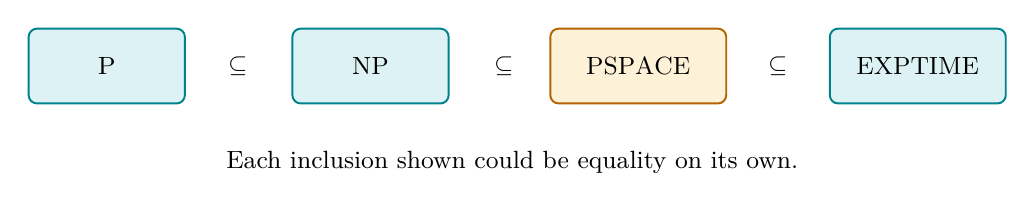
\begin{tikzpicture}[every node/.style={font=\small}]
\node[block,text width=1.75cm] (p) at (0,0) {$\mathrm P$};
\node[block,text width=1.75cm] (np) at (3.35,0) {$\mathrm{NP}$};
\node[amberblock,text width=2cm] (ps) at (6.75,0) {$\mathrm{PSPACE}$};
\node[block,text width=2cm] (ex) at (10.3,0) {$\mathrm{EXPTIME}$};
\node at (1.675,0) {$\subseteq$};
\node at (5.05,0) {$\subseteq$};
\node at (8.525,0) {$\subseteq$};
\node[align=center] at (5.15,-1.22) {Each inclusion shown could be equality on its own.};
\end{tikzpicture}\par
\end{tcolorbox}

\begin{itemize}[leftmargin=*, itemsep=3pt, topsep=4pt]
  \item \textbf{P is contained in NP.} A deterministic polynomial-time algorithm can act as the verifier.
  \item \textbf{NP is contained in PSPACE.} Enumerate all polynomial-length certificates and verify one at a time, reusing the space. The number of certificates may be exponential.
  \item \textbf{PSPACE is contained in EXPTIME.} A deterministic polynomial-space machine has at most exponentially many configurations. A halting run cannot revisit an identical configuration and then continue differently.
  \item \textbf{Completeness.} A problem is PSPACE-complete if it is in PSPACE and every problem in PSPACE reduces to it in polynomial time. A PSPACE-complete problem being in NP would imply $\mathrm{NP}=\mathrm{PSPACE}$.
\end{itemize}
The displayed containments do not resolve which adjacent classes are equal. The time hierarchy theorem does give $\mathrm{P}\subsetneq\mathrm{EXPTIME}$, so at least one adjacent inclusion in the chain is strict.

\subsection{True Quantified Boolean Formula}
\begin{tcolorbox}[defbox, title={TQBF}]
TQBF asks whether a fully quantified Boolean formula is true. An existential quantifier $\exists x$ requires at least one of $x=0,1$ to work. A universal quantifier $\forall x$ requires both to work. The quantifier order determines which choices may depend on earlier ones.
\end{tcolorbox}

\begin{tcolorbox}[examplebox, title={Quantifier order matters}]
The formula $\forall x\,\exists y\,(x\leftrightarrow y)$ is true because the choice $y=x$ works for either value of $x$. The formula $\exists y\,\forall x\,(x\leftrightarrow y)$ is false because a single fixed value of $y$ cannot match both values of $x$.
\end{tcolorbox}

\begin{tcolorbox}[formulabox, title={Depth-first evaluation of a quantified Boolean formula}]
\begin{verbatim}
If there are no quantifiers left, evaluate the matrix.
For an existential variable:
    evaluate assignments 0 and 1 as needed and take OR.
For a universal variable:
    evaluate assignments 0 and 1 as needed and take AND.
Reuse the assignment array after each recursive result.
\end{verbatim}
\end{tcolorbox}

\begin{itemize}[leftmargin=*, itemsep=2pt]
  \item \textbf{Time.} In the worst case the evaluator tries exponentially many assignments.
  \item \textbf{Working space.} The recursion depth is $n$. Store the formula and one partial assignment, and reuse the same storage when trying the next branch.
  \item \textbf{Completeness.} This shows $\mathrm{TQBF}\in\mathrm{PSPACE}$. To prove hardness, encode the reachability question for a polynomial-space machine as a quantified formula. The construction below uses one copy of the smaller reachability test per recursion level.
\end{itemize}

\subsection{Savitch's theorem and the space viewpoint}
\begin{tcolorbox}[formulabox, title={Savitch's theorem}]
For standard space bounds $s(n)\ge\log n$,
\[
\mathrm{NSPACE}(s(n))\subseteq\mathrm{DSPACE}(s(n)^2).
\]
In particular $\mathrm{NPSPACE}=\mathrm{PSPACE}$. This equality is about polynomial space. It does not imply $\mathrm{P}=\mathrm{NP}$.
\end{tcolorbox}

\textbf{Proof idea using reachability.} Let $R(a,b,k)$ mean that configuration $b$ is reachable from $a$ in at most $2^k$ steps.
\begin{enumerate}[leftmargin=*, itemsep=3pt]
  \item \textbf{Base case.} At $k=0$, check whether $a=b$ or a single legal move takes $a$ to $b$.
  \item \textbf{Recursive step.} Try each candidate midpoint $m$. Accept if both $R(a,m,k-1)$ and $R(m,b,k-1)$ hold for the same $m$.
  \item \textbf{Space bound.} Evaluate the two calls in sequence and reuse their storage. There are $2^{O(s)}$ configurations, so $O(s)$ levels suffice. Each level keeps $O(s)$ bits of configurations and counters. Total working space is $O(s^2)$.
\end{enumerate}

\textbf{Readings.} \href{https://ocw.mit.edu/courses/6-046j-design-and-analysis-of-algorithms-spring-2015/pages/lecture-notes/}{MIT 6.046J lecture notes on randomization and approximation}. Walter J. Savitch, \href{https://doi.org/10.1016/S0022-0000(70)80006-X}{Relationships Between Nondeterministic and Deterministic Tape Complexities (1970)}.

\subsection{How a quantified formula encodes reachability}
A configuration records a machine's state, head positions and working tape. For a polynomial-space machine, that record uses a polynomial number of bits $m$.

\begin{enumerate}[leftmargin=*, itemsep=3pt]
  \item \textbf{Encode one move.} The formula $R_0(x,y)$ checks whether the configurations are identical or one legal step connects them. The legal-step test has polynomial size because it checks the local update and the unchanged parts.
  \item \textbf{Check both halves with one formula.} Guess a midpoint $z$. Fresh universally quantified vectors $u,v$ select the pairs $(x,z)$ and $(z,y)$.
  \[
  \begin{aligned}
  R_k(x,y)={}&\exists z\,\forall u\,\forall v\,\big[
    \big((u=x\land v=z)\lor(u=z\land v=y)\big)\\
    &\hspace{8em}\Longrightarrow R_{k-1}(u,v)\big].
  \end{aligned}
  \]
  The antecedent is true for the two selected pairs, so each smaller reachability test must pass. For every other pair the implication is true automatically.
  \item \textbf{Bound the construction.} There are at most $2^m$ encoded configurations, so $k=m$ suffices. Each level adds polynomially many symbols and uses only one copy of $R_{k-1}$. The full formula is therefore polynomial in length.
  \item \textbf{Set the endpoints.} Start at the machine's initial configuration and existentially choose an accepting target. The formula is true exactly when the machine accepts.
\end{enumerate}

\textbf{Further reading.} \href{https://ocw.mit.edu/courses/18-404j-theory-of-computation-fall-2020/resources/lecture-18-pspace-completeness/}{MIT 18.404J lecture on PSPACE-completeness}.

\newpage
\begin{center}
  {\large\bfseries\color{myred} Quick Revision --- Module 5}\\[3pt]
  {\small\color{mydark} Approximation, Randomization and PSPACE $|$ ES-CS401}
\end{center}
\noindent{\color{myred}\rule{\linewidth}{1.2pt}}\par\vspace{4pt}

\begin{tcolorbox}[formulabox, title={Key Concepts at a Glance}]
\renewcommand{\arraystretch}{1.35}
\noindent\begin{tabularx}{\linewidth}{B{4.5cm}Y}
Minimisation ratio & $A\le\rho\,\mathrm{OPT}$ for all supported inputs. \\[3pt]
Maximisation ratio & $A\ge\mathrm{OPT}/\rho$. \\[3pt]
Matching lower bound & $\mathrm{OPT}_{\mathrm{VC}}\ge|M|$ for any matching $M$. \\[3pt]
One-sided repetition & At most $p^k$ error after $k$ independent trials under the appropriate acceptance rule. \\[3pt]
Space inclusions & $\mathrm P\subseteq\mathrm{NP}\subseteq\mathrm{PSPACE}\subseteq\mathrm{EXPTIME}$. \\[3pt]
\end{tabularx}\par
\end{tcolorbox}

\begin{tcolorbox}[defbox, title={One-Line Definitions}]
\begin{itemize}[leftmargin=*, itemsep=3pt, topsep=4pt]
  \item \textbf{Approximation ratio.} A proved factor relating feasible objective value to the optimum.
  \item \textbf{Las Vegas algorithm.} A randomized procedure with exact answers and variable running time.
  \item \textbf{Monte Carlo algorithm.} A bounded-time randomized procedure with a stated error probability.
  \item \textbf{PSPACE.} Decision problems solvable using polynomial working space.
\end{itemize}
\end{tcolorbox}

\begin{tcolorbox}[exambox, title={Frequently Asked / Viva Questions}]
\begin{enumerate}[topsep=0pt, label=\textbf{Q\arabic*.}, itemsep=5pt, leftmargin=*]
  \item \Q{What separates a heuristic from an approximation algorithm?}
    An approximation algorithm proves a solution-quality guarantee for a stated problem family.
  \item \Q{What is special about an FPTAS?}
    Its runtime is polynomial in input length and in $1/\varepsilon$.
  \item \Q{Why does the cover algorithm use a matching?}
    Each selected disjoint edge contributes a separate mandatory endpoint to any cover.
  \item \Q{Which assumption justifies shortcutting the metric TSP traversal?}
    The triangle inequality bounds the shortcut by the path it replaces.
  \item \Q{How can a randomized algorithm have worst-case and expected bounds?}
    Worst case considers the unluckiest choices. Expectation averages over the algorithm's own random choices on a fixed input.
  \item \Q{What is the worst-case time for random-pivot quicksort?}
    $\Theta(n^2)$ when each pivot is an extreme key.
  \item \Q{What is the error direction of the matrix product test?}
    It can accept a false product. A correct product always passes.
  \item \Q{Why is NP contained in PSPACE?}
    Verify polynomial-length certificates one at a time and reuse the work tape.
  \item \Q{Why can TQBF be evaluated in polynomial space?}
    A depth-first evaluation stores only the current partial assignment and recursion state.
  \item \Q{What does Savitch's theorem prove for polynomial space?}
    $\mathrm{NPSPACE}=\mathrm{PSPACE}$.
  \item \Q{Does the inclusion chain settle P versus NP?}
    The equality question remains open.
\end{enumerate}
\end{tcolorbox}

\begin{tcolorbox}[tikzbox, title={Summary Comparison}]
\par\vspace{5pt}
\begingroup
\setlength{\extrarowheight}{1pt}
\noindent\begin{tabularx}{\linewidth}{|B{3.45cm}|Y|Y|}
\hline
\textbf{Topic} & \textbf{Main goal} & \textbf{Standard example} \\ \hline
Approximation & Guaranteed feasible quality in polynomial time. & Maximal-matching vertex cover. \\ \hline
Las Vegas & Always correct with expected resource bounds. & Random-pivot quicksort. \\ \hline
Monte Carlo & Fast test with controlled error. & Freivalds' matrix product check. \\ \hline
Polynomial space & Reuse memory across an extensive search. & Depth-first TQBF evaluation. \\ \hline
\end{tabularx}\par
\endgroup
\end{tcolorbox}

\end{document}
